% id: 47-87
% book: 개념원리 기하 · 04 이차곡선
% section: 연습문제 STEP 2
% figure: crop:fig-47-87.png
% answer: $3$
% answer_source: 답지
% variant_level: 0 (원본 전사)
% 이 파일은 build.mjs 가 items.json 에서 만든다. 고칠 때는 items.json 을 고친다.
\smash{\raisebox{4.5mm}{\dmkichul{개념원리 기하 47쪽 87번}}}
\noindent\begin{minipage}[t]{0.58\linewidth}\vspace{0pt}\raggedright 오른쪽 그림과 같이 쌍곡선 $\dfrac{x^2}{2}-\dfrac{y^2}{3}=1$의 두 초점을 $\pt{F}$, $\pt{F'}$이라 하고 선분~$\pt{FF'}$을 지름으로 하는 원과 쌍곡선의 교점 중 \mbox{제$2$사분면} 위의 점을 $\pt{P}$라 할 때, 삼각형~$\pt{PF'F}$의 넓이를 구하시오.\end{minipage}\hfill\begin{minipage}[t]{0.4\linewidth}\vspace{0pt}\centering \setlength{\dmfigw}{76.6pt}\ifdim\dmfigw>\linewidth\setlength{\dmfigw}{\linewidth}\fi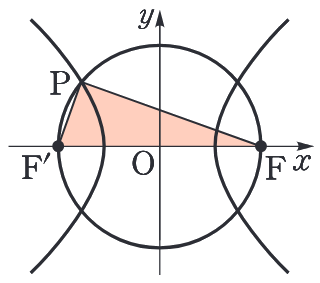
\includegraphics[width=\dmfigw]{figures/fig-47-87.png}\end{minipage}\par
